\documentclass[11pt,a4paper]{article}
\usepackage[T1]{fontenc}
\usepackage{lmodern}

% ── Packages ──────────────────────────────────────────────────────────────────
\usepackage[margin=1in]{geometry}
\usepackage{amsmath, amssymb}
\usepackage{booktabs}
\usepackage{array}
\usepackage{hyperref}
\usepackage{xcolor}
\usepackage{tikz}
\usepackage{parskip}
\usepackage{microtype}
\usepackage{enumitem}
\usepackage{caption}
\usepackage{float}
\usepackage{multirow}
\usetikzlibrary{shapes.geometric, arrows.meta, positioning, fit, backgrounds}

\hypersetup{
    colorlinks=true,
    linkcolor=blue!60!black,
    urlcolor=blue!60!black,
    citecolor=blue!60!black
}

% ── Title ─────────────────────────────────────────────────────────────────────
\title{
    \Large\textbf{Peer-Isolated Recommendation: When Content-Only}\\[4pt]
    \Large\textbf{Personalization Beats Collaborative Signal, and When It Doesn't}
}
\author{
    Bidit Das\\
    \small Independent Researcher $\mid$ Dallas, TX\\
    \small \href{mailto:biditdas18@gmail.com}{biditdas18@gmail.com}
}
\date{June 17, 2026}

% ── TikZ diagram styles ───────────────────────────────────────────────────────
\tikzset{
  mainbox/.style={
    rectangle, rounded corners=4pt,
    minimum width=8cm, minimum height=1.0cm,
    text centered, text width=7.8cm,
    font=\small\bfseries, inner sep=6pt
  },
  navybox/.style={mainbox, fill=blue!25!black, text=white},
  bluebox/.style={mainbox, fill=blue!55, text=white},
  lightbox/.style={mainbox, fill=blue!10, text=blue!30!black,
                   draw=blue!40, line width=0.8pt},
  greenbox/.style={mainbox, fill=green!35!black, text=white},
  brownbox/.style={mainbox, fill=orange!40!brown, text=white},
  warmbox/.style={mainbox, fill=orange!15, text=orange!40!brown,
                  draw=orange!40!brown, line width=0.8pt},
  purplebox/.style={mainbox, fill=violet!60!black, text=white},
  clusterbox/.style={
    rectangle, rounded corners=3pt,
    minimum width=2.3cm, minimum height=0.9cm,
    text centered, text width=2.1cm,
    font=\small\bfseries,
    fill=green!15, draw=green!40!black, line width=0.8pt,
    text=green!30!black
  },
  arrow/.style={-Stealth, thick, blue!40!black}
}

\begin{document}
\maketitle

% ── Abstract ──────────────────────────────────────────────────────────────────
\begin{abstract}
We present \textbf{Essence}, a personal embedding cluster framework for
recommendation that operates exclusively within a single user's engagement
history, without consulting cross-user interaction data. We evaluate
Essence on three datasets spanning distinct domains --- Last.fm-1K (music),
Amazon Books (e-commerce), and MovieLens-25M (film) --- against a real
collaborative-filtering baseline, a non-personalized popularity baseline, a
content-based average-embedding baseline, three recency-based baselines
(last-item, uniform-average, and exponentially-weighted retrieval), and two
hand-implemented multi-interest neural baselines (MIND~\cite{li2019},
ComiRec~\cite{cen2020}).

Essence's performance relative to these baselines is \textbf{domain-dependent}:
across the three evaluated datasets, Essence's rank among the ten evaluated
systems is associated with the strength of collaborative/popularity signal
available in the domain; establishing this as predictive would require
additional datasets and an independently-defined domain property, not one
measured post hoc via baseline performance. $K$ (the number
of interest clusters) is selected per dataset on a validation split
carved from training data, not fixed in advance --- $K=10$ for Last.fm-1K
and Amazon Books, $K=15$ for MovieLens-25M. On Amazon Books, where
collaborative and popularity baselines are structurally weak (Recall@10 of
$0.0031$ and $0.0021$ respectively), Essence ranks 3rd of 10 on Recall@10
($0.0253$): it loses only to Last-Item ($0.0311$) and is not
significantly different from Recency-Weighted ($0.0260$,
$d=-0.009$) and Avg-Last-10 ($0.0235$, which it now numerically beats). It
significantly beats collaborative filtering, popularity, content-averaging,
and both neural multi-interest baselines on Recall@10 ($d$ ranges
$0.099$--$0.282$), and significantly beats Random, Popularity, and MIND on
LT-Recall@10 specifically; it is not significantly different from CF-ItemKNN,
Content, ComiRec, Last-Item, Recency-Weighted, and Avg-Last-10 on
LT-Recall@10. On Last.fm-1K, Essence ranks 2nd of 10 on both Recall@10
($0.0281$) and LT-Recall@10 ($0.0142$); it is not significantly different
from any of the three recency-only baselines (numerically ahead of
Last-Item and Avg-Last-10, behind Recency-Weighted, $0.0304$, $d=-0.127$,
not significant).
On MovieLens-25M, where collaborative signal is strong (item-based CF
reaches $0.0850$ Recall@10, driven almost entirely by the platform's
densely-rated popular titles), Essence ranks 8th of 10 systems, losing to
collaborative filtering, popularity, and both neural baselines by the
largest effect sizes observed in this study (Cohen's $d$ down to $-0.55$).
A silhouette-stratification test, comparing Essence against
Recency-Weighted within per-user clustering-quality tertiles, finds that
$K$-means clustering is not empirically supported as the source of
Essence's advantage where an advantage exists: no stratum, on any dataset
or metric, shows Essence significantly ahead of Recency-Weighted, though
only one of sixteen clean such comparisons (MovieLens-25M's highest-silhouette
stratum on LT-Recall@10) now shows Essence significantly \emph{behind} it
either, down from six of seventeen before validation-selecting $K$. The question this
paper does not fully resolve --- how much of Essence's advantage, where it
exists, comes from clustering specifically versus recency-weighted
retrieval alone --- remains open.

We report every comparison with paired bootstrap significance testing
($10{,}000$ resamples), Benjamini--Hochberg correction for multiple
comparisons, standardized effect sizes, and BCa robustness cross-checks ---
replacing an earlier confidence-interval-overlap methodology that does not
test the quantity of interest. We also report a popularity-decile breakdown
showing that Essence's long-tail advantage, where present, is concentrated
in moderately-rare-but-observed items rather than true cold-start items, and
an artist/author-identity shortcut analysis showing that a disproportionate
share of Essence's hits come from same-artist/author candidates despite
these being a minority of its recommendations. We frame Essence not as a
universally superior candidate generator, but as a data point on when
peer-isolated, content-only personalization is and isn't the right
architectural choice.
Code: \url{https://github.com/biditdas18/essence}
\end{abstract}

% ── 1. Introduction ───────────────────────────────────────────────────────────
\section{Introduction}

Recommendation systems built on collaborative filtering (CF) derive their
signal from cross-user interaction patterns: a user's future interactions are
predicted from the behavior of users who interacted similarly in the past.
This approach performs well on standard benchmarks, particularly on metrics
dominated by popular items, but it carries a structural property worth
examining directly: items with sparse interaction histories are, by
construction, underrepresented in any signal derived from cross-user
co-occurrence. A user with a narrow, idiosyncratic taste profile
(engaging consistently with low-interaction items across a domain) receives
recommendations shaped by aggregate similarity to other users, not by the
specific combination of properties their own history reflects.

This work originated from a practical observation in music recommendation:
users with precise, narrow taste profiles are reliably steered toward
broadly popular artists that are only loosely similar, while artists matching
the specific texture of that taste remain unsurfaced regardless of how long
the user searches the catalog manually. This pattern motivated two questions
addressed here. This paper is structured as an evaluation study, not a
method-introduction paper: the central question is whether a specific
architectural choice --- $K$-means interest clustering --- provides
measurable benefit over a simpler recency-based alternative, tested under
conditions designed to give that choice its best chance to matter. First, the original motivating question: can a recommendation
signal be constructed using only a single user's own history, without any
cross-user interaction data, and if so, does it recover items that collaborative methods
structurally underrepresent? Second, a question that only becomes answerable
once the same comparison is run across multiple, structurally different
domains: under what domain conditions does this approach help versus hurt,
and is that pattern associated with properties of the domain rather than
discovered post hoc per dataset? A one- or two-dataset evaluation cannot
distinguish a domain-general advantage from a domain-specific artifact; the
three-dataset evaluation reported here (Section~\ref{sec:results}) is
designed specifically to make that distinction possible.

We propose Essence, a framework that embeds a user's consumed items into a
semantic space using a pre-trained sentence encoder, clusters them into $K$
interest profiles via $K$-means, and generates recommendations by retrieving
items similar to the centroid closest to the user's recent activity. We refer
to this as the \emph{peer-isolation property}: no cross-user interaction graph
is consulted at any stage. This is a deliberate architectural constraint, not
an oversight: it is the mechanism under test. We describe the resulting objective as depth-optimized: the goal is to retrieve items deep in a user's long-tail interest space, rather than to maximize aggregate engagement on broadly popular items.

The contributions of this work are:
\begin{enumerate}[leftmargin=*, itemsep=2pt]
  \item A \textbf{three-dataset evaluation} testing whether $K$-means
        interest clustering provides measurable benefit over a simpler
        recency-based alternative (Section~\ref{sec:results}), yielding a
        \textbf{domain-dependence finding} across three datasets spanning
        music, e-commerce, and film: Essence's relative standing among ten
        evaluated systems is associated with the strength of
        collaborative/popularity signal in the domain (establishing this as
        predictive would require additional datasets and an
        independently-defined domain property), evidenced by effect sizes
        ranging from Essence's strongest win
        (Last.fm-1K, beating Random with $d=+0.301$) to its strongest
        loss (MovieLens-25M, losing to CF-ItemKNN with $d=-0.550$).
  \item The \textbf{Essence architecture} itself: a personal recommendation
        framework requiring no collaborative signal and no supervised or cross-user
        recommender training, operating entirely on a single user's history.
  \item A \textbf{recency-based active-cluster-selection} mechanism,
        evaluated against a static mean-embedding alternative via ablation
        (Section~\ref{sec:ablation}) \emph{and} against three recency-only
        baselines that do not cluster at all (last-item, uniform-average,
        exponentially-weighted retrieval) --- the comparison against
        simpler, non-clustering alternatives that the original evaluation
        did not include.
  \item \textbf{Two hand-implemented, from-scratch multi-interest baselines}
        (MIND, following Li et al.~\cite{li2019}; ComiRec, following Cen et
        al.~\cite{cen2020}) --- neither is available in standard
        recommendation libraries, and neither original paper's benchmark
        numbers are directly comparable under this paper's evaluation
        protocol (Section~\ref{sec:setup}), so correctness is verified
        against each model's architectural specification rather than
        against a published number (Section~\ref{sec:setup} describes the
        verification methodology and a bug it caught in our own
        implementation).
  \item A \textbf{statistical-methodology correction}: paired bootstrap
        significance testing, Benjamini--Hochberg FDR correction, effect
        sizes, and BCa robustness cross-checks (Section~\ref{sec:stats-methodology}),
        replacing an earlier confidence-interval-overlap methodology,
        applied uniformly across all three datasets and sub-analyses.
\end{enumerate}

% ── 2. Related Work ───────────────────────────────────────────────────────────
\section{Related Work}
\label{sec:related}

\subsection{Collaborative Filtering}
\label{sec:cf}
Matrix factorisation methods~\cite{koren2009} and neural
extensions~\cite{he2017} remain dominant in production recommendation. Their
principal limitation is popularity bias: items with sparse interactions are
poorly represented, resulting in near-zero recall for long-tail items. CF is
optimised for the median user: it performs well on what is broadly consumed
and comparatively weakly on what is individually resonant.

\subsection{Multi-Interest Retrieval}
\label{subsec:multi}

MIND~\cite{li2019} introduced dynamic routing to extract multiple interest
capsules from a user's interaction history, explicitly addressing the failure
of a single user vector to represent diverse tastes. ComiRec~\cite{cen2020}
extended this with explicit diversity controls at serving time.

Essence shares the multi-interest intuition with MIND and ComiRec, the
recognition that a user's preferences cannot be collapsed into a single
vector. However, the similarity ends at the surface. The distinction operates
at two levels.

\textbf{Data level.} MIND and ComiRec require population-level interaction
graphs. Their dynamic routing is trained on millions of (user, item,
interaction) triples across the full user base. Cross-user behavioural data
is not optional: it is the mechanism by which interest capsules are learned.
Essence requires no data from any other user, ever. The $K$-means centroids
are derived entirely from one user's own history.

\textbf{Representation level.} Because MIND's item embeddings are trained on
co-occurrence patterns across users, what an item \emph{means} in that space
is partly defined by who else interacted with it. An obscure track heard by very few
users is underrepresented or invisible in that embedding space, as its
co-occurrence signal is too sparse to be learned reliably. Essence uses a
pre-trained sentence encoder on item metadata only. The embedding captures metadata-derived semantic information about the item,
independent of how many people have interacted with it. A singleton item can
be embedded as readily as a chart-topping one; the quality of that
representation depends on how informative the item's metadata is, not on its
interaction count.

This distinction suggests a hypothesis: Essence should recover long-tail
items at higher rates than systems whose embeddings are shaped by
co-occurrence sparsity. We test this directly against hand-implemented
MIND and ComiRec baselines (Section~\ref{sec:setup}), and the result is
more qualified than the hypothesis alone predicts: Essence significantly
outperforms both on Amazon Books, but on MovieLens-25M both neural
baselines substantially outperform Essence instead, by some of the
largest effect sizes observed in this study
(Section~\ref{sec:domain-dependence}). The data-level and
representation-level distinctions described above are architectural facts
regardless of outcome; whether they translate into a long-tail recovery
advantage in practice depends on domain conditions, not on the
architectural distinction alone.

Table~\ref{tab:comparison} summarises the architectural distinctions between
Essence, MIND, ComiRec, and standard CF.

\begin{table}[H]
\centering
\caption{Architectural comparison: Essence vs.\ prior systems.
         The primary distinction is not the clustering mechanism,
         it is the data requirement and what each system is structurally
         able to score. All four systems are empirically evaluated in this work
         (Section~\ref{sec:results}), which reports the domain-dependent
         long-tail recovery result in full.}
\label{tab:comparison}
\begin{tabular}{lcccc}
\toprule
\textbf{Property} & \textbf{CF} & \textbf{MIND} & \textbf{ComiRec}
                  & \textbf{Essence} \\
\midrule
Cross-user data required    & Yes  & Yes  & Yes  & \textbf{No}  \\
Multiple interest profiles  & No   & Yes  & Yes  & \textbf{Yes} \\
Gradient-based training required & No  & Yes  & Yes  & \textbf{No}  \\
Can score zero-interaction items & No & No & No & \textbf{Yes} \\
Embedding source            & Co-occurrence & Co-occurrence
                            & Co-occurrence & \textbf{Item metadata} \\
\bottomrule
\end{tabular}
\end{table}

\subsection{Session-Based and Content-Based Methods}
BERT4Rec~\cite{sun2019} and GRU4Rec~\cite{hidasi2016} model sequential user
behaviour using transformer and recurrent architectures, capturing short-term
context effectively. Content-based filtering relies on item feature similarity
without interaction logs but typically averages preferences into a single
vector, losing intra-user diversity.

Essence occupies a complementary position: it captures intra-user diversity
(like multi-interest methods) without cross-user interaction data (like content-based
methods), using simple interpretable clustering rather than a trained
sequential model. We acknowledge that BERT4Rec offers richer sequential
modelling in high-interaction settings; Essence targets privacy-first,
low-infrastructure deployment contexts where such models are not viable.

\subsection{Reproducibility and Progress in Recommender Systems Research}

Ferrari Dacrema et al.~\cite{dacrema2019} showed that a majority of neural
recommendation papers at top venues failed to outperform simple, well-tuned
non-neural baselines when those baselines were given a fair tuning budget,
and that a substantial fraction of claimed improvements did not reproduce
under careful re-evaluation. A follow-up analysis~\cite{dacrema2021}
extended this finding across a broader set of papers and venues, identifying
weak baselines, inconsistent evaluation protocols, and selective reporting
as recurring, systemic causes of inflated claims of progress in the field.
This paper's own findings are consistent with, and extend, that line of
critique to a different architecture family: content-only,
no-cross-user-pooling personalization. Essence's headline long-tail
advantage survives paired bootstrap significance testing on Amazon Books
but is directional and not statistically significant on the smaller
Last.fm-1K, and on MovieLens-25M --- a domain with strong collaborative
signal --- Essence loses to collaborative filtering, popularity, and both
neural multi-interest baselines by the largest effect sizes observed
anywhere in this study (Section~\ref{sec:domain-dependence}). This is the
discipline Ferrari Dacrema et al.\ call for: a fair, statistically grounded
comparison against strong, simple baselines, with mixed results reported
alongside favorable ones.

% ── 3. The Essence Framework ──────────────────────────────────────────────────
\section{The Essence Framework}
\label{sec:framework}

\subsection{Notation}

Table~\ref{tab:notation} defines all mathematical notation used in this
section. For each symbol a plain-English equivalent is provided.

\begin{table}[H]
\centering
\caption{Notation Legend}
\label{tab:notation}
\begin{tabular}{ll}
\toprule
\textbf{Symbol} & \textbf{Plain-English Meaning} \\
\midrule
$H_u$                     & All items user $u$ has consumed (full history) \\
$i_1, i_2, \ldots$        & Individual items in the user's history, in order \\
$\phi(i)$                 & Embedding of item $i$, a 384-dim vector describing its content \\
$E_u$                     & All embeddings stacked into a matrix, one row per item \\
$K$                       & Number of interest clusters (validation-selected per dataset: $K=10$ Last.fm-1K/Amazon Books, $K=15$ MovieLens-25M) \\
$c_1, \ldots, c_K$        & The $K$ cluster centres, one per interest profile \\
$c_k^*$                   & Active cluster centre, closest to the user's recent activity \\
$\mu(\cdot)$              & Mean (average) of a set of vectors \\
$\cos(\mathbf{a},\mathbf{b})$ & Cosine similarity: how alike two vectors are \\
$I \setminus H_u$         & All items the user has \emph{not} yet consumed, the candidate pool \\
$R_u$                     & Final ranked recommendation list for user $u$ \\
$M$                       & Number of recommendations to return (we use $M=10$) \\
\bottomrule
\end{tabular}
\end{table}

\subsection{Problem Formulation}
Given a user's history $H_u$ (all items they have consumed), the
goal is to produce a ranked list $R_u \subseteq I \setminus H_u$ of items
they have not yet consumed but are likely to enjoy. Essence accomplishes this
using only $H_u$ and a shared embedding function $\phi: I \to \mathbb{R}^d$.
No data from any other user is used at any stage.

\subsection{Item Embedding}
Each item is described by a short text string encoding its content properties.
For music: track name and artist name. For books: title and author name. We
convert this text into a 384-dimensional vector using the pre-trained sentence
encoder \texttt{all-MiniLM-L6-v2}~\cite{reimers2019,wang2020}. Items that are
semantically similar produce similar vectors; items that are stylistically
distant produce different vectors. Critically, this embedding is derived from item metadata text, not from
interaction patterns. A niche item can be embedded as readily as a popular
one; representation quality depends on the informativeness of the metadata
rather than on interaction frequency. All embeddings are computed once offline
and cached.

Formally, $\phi(i)$ is the embedding of item $i$. For user $u$ with history
$H_u = \{i_1, \ldots, i_n\}$ we compute the embedding matrix
$E_u \in \mathbb{R}^{n \times d}$, where each row is the embedding of one
item.

\subsection{Interest Profile Clustering}
We apply $K$-means clustering to $E_u$ with a per-dataset $K$ (selection
procedure below), yielding centroids $\{c_1, \ldots, c_K\}$. Each centroid
represents a distinct interest profile: the semantic centre of gravity of
one coherent facet of the user's taste. A user who consumes jazz, indie
rock, and ambient electronica might, for example, end up with one centroid
per genre under $K=3$. The $K$ centroids together form the user's interest
profile $P_u = \{c_1, \ldots, c_K\}$.

This is the core differentiator from average-embedding approaches. The mean
of all embeddings collapses all interests into a single blurred point that
sits between clusters and represents none of them well. $K$-means preserves
the separation between interest modes, enabling targeted retrieval against
each mode independently.

$K$ is selected per dataset on a validation split carved from the
training data (the last 20\% of each user's chronological training
history; the held-out test set is never touched during selection). $K$
is swept over $\{2, 3, 4, 5, 8, 10, 15, 20, 30, 50\}$ (log-spaced above
$K=8$), and the sweep for a given dataset stops at the first $K$ where
either (i) validation Recall@10 improves by less than 2\% relative to
the previous tested $K$, or (ii) the mean number of items per cluster
(training items per user, divided by $K$, averaged over users with
enough history to cluster) falls below 3 --- whichever triggers first.
The selected $K$ is the validation-Recall@10-maximizing point among the
values tested before the stopping rule fires. This yields $K=10$ for
Last.fm-1K and Amazon Books, and $K=15$ for MovieLens-25M. One
methodological note on how the sweep was conducted: the stopping rule
was applied moving forward from $K=8$ (an earlier, already-reported
checkpoint in this project's revision history) rather than from $K=2$;
applied retroactively to the $K\in\{2,\ldots,5\}$ region, the rule would
in fact have triggered earlier for Amazon Books and MovieLens-25M, since
validation Recall@10 dips slightly between some of those early,
closely-spaced values before climbing again at higher $K$. We report
this plainly as a scope decision --- continuing the already-established
$K=8$ checkpoint forward, rather than restarting the rule from $K=2$ ---
not a result the stopping rule itself produced.

For users with fewer than $K$ items, Essence falls back to the content
baseline (single mean embedding).

\subsection{Active Cluster Selection}
\label{subsec:active}
At inference time, Essence selects the active centroid $c_k^*$ as the
cluster centre closest to the mean embedding of the user's $r$ most recent
training-set interactions, ordered chronologically (default $r=10$):

\begin{equation}
  c_k^* \;=\; \arg\min_k \;\bigl\| c_k - \mu\!\left(\phi(h_{n-r+1}), \ldots, \phi(h_n)\right) \bigr\|_2
  \label{eq:active}
\end{equation}

This mechanism assumes recent activity is informative about which interest
cluster is currently active. We test this assumption directly via ablation
(Section~\ref{sec:ablation}): replacing the recency-based query with the mean
embedding of the user's entire training history degrades long-tail recall
substantially on Last.fm-1K, indicating that recency carries signal
beyond what the $K$-means clustering step alone provides. The ablation is
the basis for retaining recency as the default mechanism.

\subsection{Recommendation Generation}
Given the active centroid $c_k^*$, Essence retrieves the top-$M$ unseen
items by cosine similarity:

\begin{equation}
  R_u \;=\; \operatorname{top-}M\;\bigl\{\, i \in I \setminus H_u \;:\;
  \cos\!\left(\phi(i),\, c_k^*\right) \bigr\}
  \label{eq:reco}
\end{equation}

This retrieval step operates entirely in embedding space with no collaborative
signal. An item's probability of appearing in $R_u$ is determined solely by
its latent similarity to the user's current interest cluster, not by how
many other users have interacted with it.

\subsection{Architecture Overview}

Figure~\ref{fig:pipeline} illustrates the full Essence pipeline from raw user
history to final recommendations.

\begin{figure}[H]
\centering
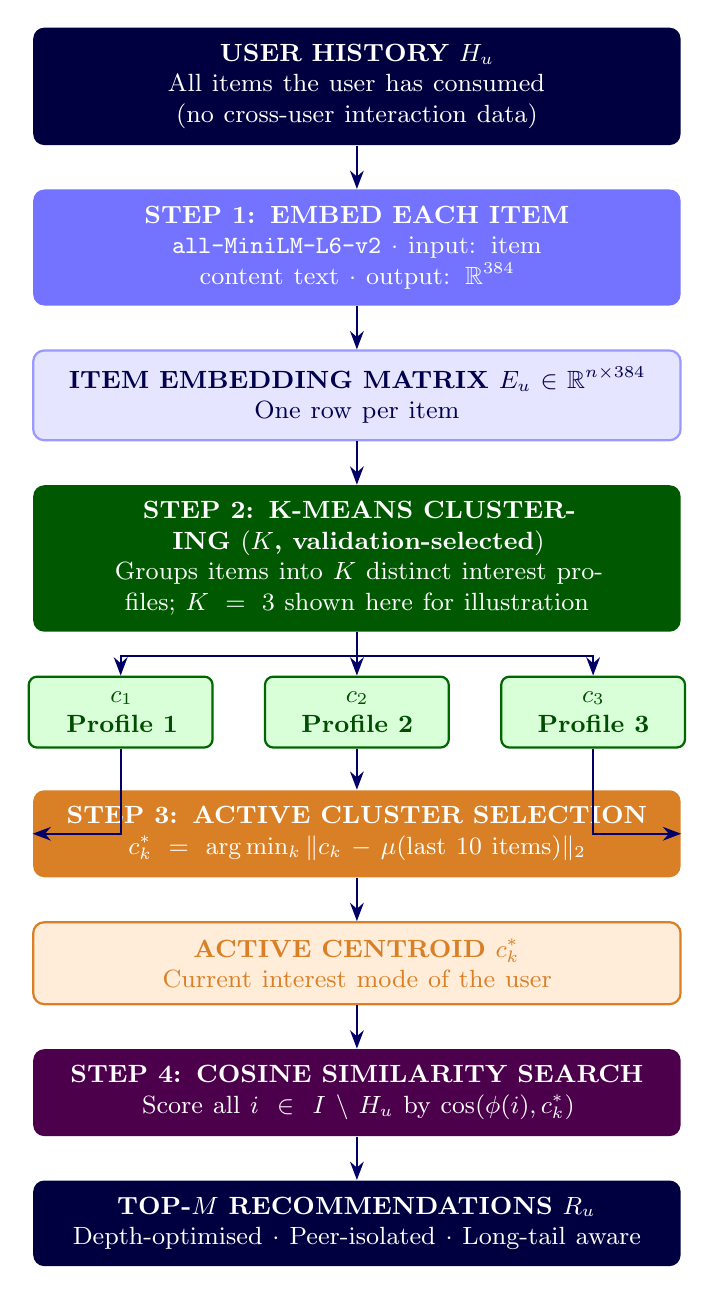
\begin{tikzpicture}[node distance=0.55cm, every node/.style={align=center}]

  \node[navybox]  (hist)   {USER HISTORY $H_u$\\
                             \normalfont\small All items the user has consumed
                             (no cross-user interaction data)};

  \node[bluebox,  below=of hist]  (emb)
        {STEP 1: EMBED EACH ITEM\\
         \normalfont\small \texttt{all-MiniLM-L6-v2} $\cdot$
         input: item content text $\cdot$ output: $\mathbb{R}^{384}$};

  \node[lightbox, below=of emb]   (mat)
        {ITEM EMBEDDING MATRIX $E_u \in \mathbb{R}^{n \times 384}$\\
         \normalfont\small One row per item};

  \node[greenbox, below=of mat]   (km)
        {STEP 2: K-MEANS CLUSTERING $(K$, validation-selected$)$\\
         \normalfont\small Groups items into $K$ distinct interest profiles; $K=3$ shown here for illustration};

  \node[clusterbox, below=of km, xshift=-3.0cm] (c1) {$c_1$\\Profile 1};
  \node[clusterbox, below=of km]                (c2) {$c_2$\\Profile 2};
  \node[clusterbox, below=of km, xshift=+3.0cm] (c3) {$c_3$\\Profile 3};

  \node[brownbox, below=2.0cm of km] (active)
        {STEP 3: ACTIVE CLUSTER SELECTION\\
         \normalfont\small $c_k^* = \arg\min_k \|c_k - \mu(\text{last 10 items})\|_2$};

  \node[warmbox,  below=of active] (ck)
        {ACTIVE CENTROID $c_k^*$\\
         \normalfont\small Current interest mode of the user};

  \node[purplebox, below=of ck]   (ann)
        {STEP 4: COSINE SIMILARITY SEARCH\\
         \normalfont\small Score all $i \in I \setminus H_u$ by
         $\cos(\phi(i), c_k^*)$};

  \node[navybox,  below=of ann]   (out)
        {TOP-$M$ RECOMMENDATIONS $R_u$\\
         \normalfont\small Depth-optimised $\cdot$
         Peer-isolated $\cdot$ Long-tail aware};

  \draw[arrow] (hist)   -- (emb);
  \draw[arrow] (emb)    -- (mat);
  \draw[arrow] (mat)    -- (km);
  \draw[arrow] (km.south) -- ++(0,-0.3) -| (c1.north);
  \draw[arrow] (km.south) -- ++(0,-0.3) -| (c2.north);
  \draw[arrow] (km.south) -- ++(0,-0.3) -| (c3.north);
  \draw[arrow] (c1.south) |- (active.west);
  \draw[arrow] (c2.south) -- (active.north);
  \draw[arrow] (c3.south) |- (active.east);
  \draw[arrow] (active) -- (ck);
  \draw[arrow] (ck)     -- (ann);
  \draw[arrow] (ann)    -- (out);

\end{tikzpicture}
\caption{Essence recommendation pipeline. No cross-user interaction data is consulted at
any stage (peer-isolation property).}
\label{fig:pipeline}
\end{figure}

% ── 4. Experimental Setup ─────────────────────────────────────────────────────
\section{Experimental Setup}
\label{sec:setup}

\subsection{Datasets}

\textbf{Last.fm-1K (music).} Contains listening histories from 992 users
across approximately 19 million events~\cite{celma2010}. After filtering to
users with 50--500 unique track interactions and removing duplicate
(user, track) pairs, our evaluation subset contains 99~users and 22{,}767
unique tracks --- this is the full filtered dataset, not a subsample: no
further sampling is applied after the interaction-count filter. A positive
interaction is any recorded play; there is no minimum play count or other
threshold beyond the 50--500 per-user interaction-count filter. Item
embeddings are built from track title + artist name (metadata only; no
interaction signal enters the embedding).

\textbf{Amazon Books (e-commerce).} The Amazon Reviews 2023 Books 5-core
dataset~\cite{hou2024}, which guarantees every user and item has at least
5 global interactions. After filtering to users with 20--200 unique item
interactions and subsampling to 2{,}000 users (seed~42), our evaluation
subset contains 2{,}000 users and 61{,}727 unique items. Item embeddings use
title + author name + description, following the same metadata-only
approach as Last.fm-1K. A positive interaction is any rating or review in
the 5-core file; no minimum star-rating value is required (a 1-star and a
5-star rating both count equally as an interaction). The 20--200-interaction filter and the 2{,}000-user
subsample size are applied identically, with the same seed, to MovieLens-25M
below --- fixed a priori and held constant across both datasets rather than
tuned per dataset, to keep the evaluation (including MIND/ComiRec training
and the full bootstrap/FDR suite) computationally tractable at the same
scale on both.

\textbf{MovieLens-25M (film).} A 2{,}000-user subsample (seed~42, same
20--200-interaction filter and sampling convention as Amazon Books) drawn
from the MovieLens-25M ratings dataset. Item text is built from title +
genres, plus overview text from The Movie Database (TMDb) when available;
of $7{,}724$ candidate items identified from the sampled users'
interactions, $7{,}654$ had a TMDb record successfully fetched at all
($99.1\%$), and these form the final catalog --- the remaining $70$ items,
for which the TMDb API lookup itself failed, are excluded from the
candidate pool entirely (not merely missing overview text). Within the
$7{,}654$ fetched items, any with an empty overview field fall back to
title + genres only rather than being dropped. Our
evaluation subset contains 2{,}000 users and $7{,}654$ catalog items. A
positive interaction is any rating in the sampled ratings file; no minimum
star-rating value is required.

\textbf{Data attribution.} This product uses the TMDb API but is not
endorsed or certified by TMDb.

\subsection{Train/Test Split}
For each user on all three datasets, interactions are sorted chronologically and
split per-user: the first 80\% form the training set, and the final 20\%
form the test set. This chronological split is required for internal
consistency with the active-cluster-selection mechanism
(Section~\ref{subsec:active}), which defines ``recent'' interactions in terms
of training-set recency; a random split would make this definition
incoherent, since a randomly held-out test item could chronologically
precede items retained in training. The split is computed independently
per user, with no shared global time cutoff across users: each user's
train/test boundary is defined purely by their own interaction history,
not by any dataset-wide date. This preserves within-user chronology but
does not enforce a global temporal cutoff; possible cross-user temporal
leakage for population-based baselines (CF, Popularity) --- an item's
co-occurrence signal can include other users' interactions that occurred,
in wall-clock time, after a given user's personal train/test cutoff --- is
therefore a limitation of this evaluation protocol, not eliminated by it
(Section~\ref{sec:limitations}).

Item embeddings are computed once, offline, over the full item catalog
(train $\cup$ test), so that no test item is excluded from the retrieval
candidate pool due to missing embedding coverage. This is independent of the
train/test split decision and applies identically under either splitting
strategy.

\subsection{Long-Tail Definition}
Long-tail items are those with insufficient interaction signal for
collaborative filtering to represent reliably. We define long-tail
operationally per dataset, anchored to each dataset's interaction density:

\begin{itemize}[leftmargin=*, itemsep=3pt]
  \item \textbf{Last.fm-1K.} Items with a training-set interaction count of
        exactly~1 (\emph{singleton tracks}): $16{,}761$ of the $18{,}679$
        items appearing in the training set ($89.7\%$). The full candidate
        pool (train~$\cup$~test) is $22{,}767$ tracks.
  \item \textbf{Amazon Books.} Items with a training-set interaction count of
        exactly~1 (\emph{singleton items}): $42{,}878$ of the $50{,}924$
        items appearing in the training set ($84.2\%$). The full candidate
        pool (train~$\cup$~test) is $61{,}727$ items. Despite the 5-core
        guarantee of at least~5 global interactions, subsampling to
        2{,}000 users reduces most items to a single observed interaction
        in the subset's training split.
  \item \textbf{MovieLens-25M.} Items with a training-set interaction count
        of exactly~1: $2{,}337$ of the $6{,}745$ items appearing in the
        training set ($34.6\%$). Unlike Last.fm-1K and Amazon Books, where
        singleton items concentrate at the rare-popularity end of the
        catalog (deciles 3--9), MovieLens-25M's singletons concentrate more
        centrally, in deciles 2--5 ($32.7\%$ and $32.8\%$ of all singletons
        falling in deciles 3 and 4 alone) --- a dataset-specific difference
        in decile geometry, not a methodological inconsistency.
\end{itemize}

LT-Recall@10 is computed only over users with at least one long-tail test
item; the remaining users contribute no LT-Recall@10 observation for that
metric. Eligible users: 92 of 99 on Last.fm-1K, 1{,}292 of 2{,}000 on
Amazon Books, 490 of 2{,}000 on MovieLens-25M.

\textbf{Generalisation principle.} The long-tail threshold should be set at
the point where collaborative filtering loses reliable signal, empirically
where item interaction count falls below the minimum required for stable
co-occurrence estimation. On Last.fm-1K and Amazon Books, the singleton
threshold (train interaction count~$= 1$) proved the most meaningful
boundary: alternative thresholds either collapsed toward the full catalog
(losing discriminative power) or excluded too few items; the same
threshold was applied to MovieLens-25M without modification and produced
a comparably non-degenerate singleton population ($34.6\%$ of training-set
items), though alternative thresholds were not separately swept on this
third dataset. The key invariant
is that long-tail items are defined on the \emph{training set only}, after
the train/test split, ensuring no leakage from held-out interactions into the
long-tail classification.

LT-Recall@10 is computed only over test items falling in the long-tail set.
Users with no long-tail test items are excluded from this metric.

\subsection{Systems Compared}
\begin{itemize}[leftmargin=*, itemsep=3pt]
  \item \textbf{Random.} Recommends $M$ items drawn uniformly from the
        unseen candidate pool. Establishes the floor against which all other
        systems are compared.
  \item \textbf{Popularity.} Recommends the $M$ globally most-interacted-with
        items the user has not consumed. A non-personalized baseline;
        included for comparison but not treated as collaborative filtering.
  \item \textbf{CF (ItemKNN).} An item-based collaborative filtering
        baseline, computed via cosine similarity over
        the sparse user-item interaction matrix. Recommends items most
        similar, by co-occurrence pattern, to items the user has already
        consumed. No neighbor-count cutoff or shrinkage term is applied: a
        candidate's score is the cosine-weighted sum over all training items
        with any co-occurring user, i.e.\ full-neighborhood ($k=\infty$)
        ItemKNN rather than a truncated top-$k$ variant.
  \item \textbf{Content (Average Embedding).} Computes the mean of all the
        user's item embeddings and retrieves the $M$ most similar unseen
        items by cosine similarity. Standard content-based filtering without
        interest decomposition.
  \item \textbf{Essence (validation-selected $K$).} Clusters user history into
        $K$ centroids ($K=10$ Last.fm-1K/Amazon Books, $K=15$ MovieLens-25M;
        selection procedure in Section~\ref{sec:framework}), selects the
        active centroid by Equation~\eqref{eq:active}, and retrieves top-$M$
        unseen items by Equation~\eqref{eq:reco}.
  \item \textbf{Last-Item.} Recommends the $M$ unseen items most similar,
        by cosine similarity, to the single most recent item in the user's
        training history. The simplest possible recency-based retrieval:
        no averaging, no decay, no clustering.
  \item \textbf{Avg-Last-10.} Recommends the $M$ unseen items most similar
        to the uniform mean embedding of the user's last 10 training
        interactions.
  \item \textbf{Recency-Weighted.} Recommends the $M$ unseen items most
        similar to an exponentially-decay-weighted mean of the user's last
        10 training interactions (decay $=0.9$; the most recent item
        receives weight $\propto 0.9^{0}$, the tenth-most-recent
        $\propto 0.9^{9}$, renormalized to sum to 1). Last-Item,
        Avg-Last-10, and Recency-Weighted use exactly the same item
        embeddings as Content and Essence; the only difference across all
        five is how the query vector is constructed from recent history.
  \item \textbf{MIND.} A hand-implemented dynamic-routing multi-interest
        network, following Li et al.'s original architecture~\cite{li2019}
        ($K=4$ interest capsules, a bilinear routing matrix shared across
        capsules, 3 routing iterations, routing logits initialized
        $b \sim \mathcal{N}(0, 0.01^2)$). Neither MIND nor ComiRec is
        available in standard recommendation libraries, and neither
        original paper's reported benchmark numbers are directly
        comparable here: Li et al.\ benchmark on an internal industrial
        dataset and Amazon Books, and Cen et al.\ on Amazon Books, Taobao,
        and a mobile-Taobao set, all under sampled-negative evaluation
        (one positive against roughly 100--1{,}000 negatives); none report
        Last.fm-1K at all, and Amazon Books here uses this paper's own
        2{,}000-user subsample, full-catalog ranking, and no negative
        sampling (Section~\ref{sec:setup}) --- a harder protocol under
        which lower absolute recall than the original papers' is expected
        by construction, not evidence of a broken implementation. We
        therefore verify correctness against each model's architectural
        specification directly, rather than by matching a published
        benchmark number: a synthetic conformance test for MIND's routing
        mechanism, and a directional sanity check (Recall@10 convincingly
        above Random and Popularity, and within a plausible order of
        magnitude of the published ranges once the protocol difference is
        accounted for) applied to both models' final results. The
        conformance test caught a symmetry-breaking bug in \emph{our
        implementation} --- not a flaw in the original architecture: an
        initial version zero-initialized $b$, which, because the shared
        bilinear matrix makes the pre-routing representation identical
        across capsules, guaranteed every capsule updated identically,
        silently collapsing the model's effective interest count to 1
        regardless of the nominal $K$. The test
        (\texttt{test\_mind\_\allowbreak routing.py}) caught this before
        any number reported here was generated; catching a real,
        non-obvious bug is the evidence the verification method works, not
        just a disclosed limitation.
  \item \textbf{ComiRec (SA).} A hand-implemented self-attentive
        multi-interest network, following Cen et al.'s original
        architecture~\cite{cen2020} ($K=4$ interest capsules, per-capsule
        learned query projections implemented as a single $K$-output
        linear layer, softmax attention over sequence positions). ComiRec's
        per-capsule projections are independently initialized rather than
        derived from a shared matrix, so it has no equivalent to MIND's
        symmetry-breaking failure mode and was checked with the directional
        sanity check described above rather than a dedicated conformance
        test; no comparable bug was found.
  \item \textbf{MIND/ComiRec training.} Both models share the same fixed,
        untuned training procedure, taken from the original papers'
        recommended ranges rather than grid-searched: Adam optimizer,
        learning rate $10^{-3}$, batch size 64, max sequence length 50, up
        to 50 epochs with early stopping (patience 5) on validation loss
        over each user's held-out last training interaction. The training
        objective is a sampled-softmax loss: the positive item's score plus
        100 uniform-random negative items' scores (drawn item-uniformly,
        excluding the padding index) are passed through a cross-entropy
        loss against the positive. Item and interest-capsule embeddings are
        384-dimensional, matching the shared \texttt{all-MiniLM-L6-v2}
        embedding space used by every other system.
\end{itemize}

Both MIND and ComiRec are trained across 3--4 seeds per dataset to confirm
the domain-dependence pattern (Section~\ref{sec:domain-dependence}) is not
seed-specific (Section~\ref{sec:multiseed}).

\subsection{Metrics}

\textbf{What we are measuring.} Each system produces a ranked list of 10
recommended items per user. We know which items that user actually consumed
in the test set (ground truth). The evaluation asks: how much of that ground
truth did the system recover?

This is a retrieval problem, not a classification problem. All systems are
evaluated against the \emph{full item catalog} with no negative sampling,
following the full-ranking evaluation protocol~\cite{krichene2020}. Absolute
recall values are low by construction under this protocol: the meaningful
signal is relative comparison across systems evaluated under identical
conditions.

\begin{itemize}[leftmargin=*, itemsep=3pt]
  \item \textbf{Recall@10.} Fraction of the user's test items appearing in
        the top-10 recommendations.
        \[
          \text{Recall@10} = \frac{|\,R_u \cap \text{Test}_u\,|}{|\,\text{Test}_u\,|}
        \]
        Example: 20 test items, 2 hits in top-10. Recall@10 $= 0.10$.
        Averaged across all users.

  \item \textbf{Long-Tail Recall@10 (LT-Recall@10).} Recall@10 restricted to
        singleton test items only.
        \[
          \text{LT-Recall@10} =
          \frac{|\,R_u \cap \text{LT-Test}_u\,|}{|\,\text{LT-Test}_u\,|}
        \]
        A long-tail hit means the system recommended a niche item that this
        specific user genuinely consumed, without any popularity signal
        and without any other user's behaviour to guide it. This metric
        directly tests Essence's core hypothesis.

  \item \textbf{Lift over random.} Recall@10 divided by expected random
        recall ($M / |I|$). Normalises for candidate pool size and makes
        cross-dataset comparison interpretable.
\end{itemize}

\subsection{Implementation}
All systems implemented in Python~3.11. Embeddings via
\texttt{sentence-transformers} (\texttt{all-MiniLM-L6-v2}, 384~dims).
$K$-means via \texttt{scikit-learn} (\texttt{n\_init=10},
\texttt{random\_state=42}). MIND and ComiRec are implemented from scratch
in PyTorch, since neither is available in RecBole or comparable standard
recommendation libraries; both are trained per dataset.
All ranking steps break score ties deterministically (stable sort by item
index), so reported results are exactly reproducible; this matters for sparse
baselines such as CF (ItemKNN), where many candidate items receive identical
scores.
Significance testing methodology (paired bootstrap, FDR correction, effect
sizes, BCa cross-checks) is described once, in
Section~\ref{sec:stats-methodology}, and applied identically across all
three datasets rather than being re-derived per dataset.
Code available at:
\url{https://github.com/biditdas18/essence}

% ── 5. Results ────────────────────────────────────────────────────────────────
\section{Results}
\label{sec:results}

\subsection{Headline Results, All Three Datasets}
\label{sec:headline}

Table~\ref{tab:headline-recall} and Table~\ref{tab:headline-lt} report
Recall@10 and LT-Recall@10 for all ten systems on all three datasets (99
users on Last.fm-1K, 2{,}000 users on Amazon Books, 2{,}000 users on
MovieLens-25M; chronological 80/20 split per user throughout; catalog
sizes and long-tail definitions in Section~\ref{sec:setup}). Essence's
rank among the ten systems is noted next to its own value in each column.

\begin{table}[H]
\centering
\caption{Headline Recall@10, all three datasets ($M=10$). Best result per
         dataset in \textbf{bold}. Essence's rank (of 10) is shown in
         parentheses. Essence uses its validation-selected $K$ per dataset
         ($K=10$ Last.fm-1K/Amazon Books, $K=15$ MovieLens-25M;
         Section~\ref{sec:framework}).}
\label{tab:headline-recall}
\begin{tabular}{lccc}
\toprule
\textbf{System} & \textbf{Last.fm-1K} & \textbf{Amazon Books} & \textbf{MovieLens-25M} \\
\midrule
Random                   & 0.0001 & 0.0001 & 0.0012 \\
Popularity               & 0.0023 & 0.0021 & 0.0517 \\
CF (ItemKNN)             & 0.0018 & 0.0031 & \textbf{0.0850} \\
Content (Avg Embedding)  & 0.0038 & 0.0173 & 0.0043 \\
Last-Item                & 0.0265 & \textbf{0.0311} & 0.0091 \\
Avg-Last-10              & 0.0252 & 0.0235 & 0.0064 \\
Recency-Weighted         & \textbf{0.0304} & 0.0260 & 0.0076 \\
MIND                     & 0.0078 & 0.0052 & 0.0423 \\
ComiRec (SA)             & 0.0137 & 0.0056 & 0.0706 \\
\textbf{Essence (val.\ $K$)} & 0.0281 (2nd) & 0.0253 (3rd) & 0.0053 (8th) \\
\bottomrule
\end{tabular}
\end{table}

\begin{table}[H]
\centering
\caption{Headline LT-Recall@10, all three datasets ($M=10$). Best result
         per dataset in \textbf{bold}. Essence's rank (of 10) is shown in
         parentheses. Essence uses its validation-selected $K$ per dataset,
         as above.}
\label{tab:headline-lt}
\begin{tabular}{lccc}
\toprule
\textbf{System} & \textbf{Last.fm-1K} & \textbf{Amazon Books} & \textbf{MovieLens-25M} \\
\midrule
Random                   & 0.0000 & 0.0000 & 0.0000 \\
Popularity               & 0.0000 & 0.0000 & 0.0000 \\
CF (ItemKNN)             & 0.0000 & 0.0137 & 0.0037 \\
Content (Avg Embedding)  & 0.0029 & 0.0124 & 0.0020 \\
Last-Item                & 0.0064 & \textbf{0.0215} & 0.0031 \\
Avg-Last-10              & 0.0134 & 0.0196 & 0.0026 \\
Recency-Weighted         & \textbf{0.0151} & 0.0179 & \textbf{0.0046} \\
MIND                     & 0.0021 & 0.0057 & 0.0000 \\
ComiRec (SA)             & 0.0050 & 0.0121 & 0.0014 \\
\textbf{Essence (val.\ $K$)} & 0.0142 (2nd) & 0.0207 (2nd) & 0.0030 (4th) \\
\bottomrule
\end{tabular}
\end{table}

Essence's standing is not uniform across datasets. On Amazon Books it is
3rd of 10 on Recall@10 and 2nd of 10 on LT-Recall@10 (behind only
Last-Item on both metrics; not significantly different from
Recency-Weighted on Recall@10 --- Section~\ref{sec:stats-methodology});
on Last.fm-1K it is 2nd of 10 on both Recall@10 and LT-Recall@10, not
significantly different from any of the three recency-only baselines
(numerically ahead of Last-Item and Avg-Last-10, behind Recency-Weighted);
on MovieLens-25M it is 8th of 10 on
Recall@10, ahead of only Content and Random, and 4th on LT-Recall@10.
Full significance testing for every pairwise comparison in these tables is
reported in Section~\ref{sec:stats-methodology}.

\subsection{The Domain-Dependence Pattern}
\label{sec:domain-dependence}

Essence's rank is not randomly scattered across the three datasets: it is
associated with the strength of collaborative and popularity signal
available in each domain, measured by how well the non-personalized
Popularity baseline and the CF (ItemKNN) baseline perform in that domain
(Table~\ref{tab:domain-dependence}). Establishing this association as
predictive would require additional datasets and an independently-defined
domain property, not one measured post hoc via baseline performance, as
here.

\begin{table}[H]
\centering
\caption{Essence's rank (of 10 systems, Recall@10) against the strength of
         collaborative/popularity signal in each domain.}
\label{tab:domain-dependence}
\begin{tabular}{@{}lp{5.3cm}p{4.7cm}@{}}
\toprule
\textbf{Dataset} & \textbf{Essence rank} & \textbf{CF / Popularity signal} \\
\midrule
Amazon Books    & 3rd (beats 7, ties Recency-Weighted, loses to Last-Item) & Weak (CF $0.0031$, Popularity $0.0021$) \\
Last.fm-1K      & 2nd (beats 8, ties Recency-Weighted) & Weak (CF $0.0018$, Popularity $0.0023$) \\
MovieLens-25M   & 8th (beats only Content, Random) & \textbf{Strong} (CF/Pop./ComiRec/MIND are top 4) \\
\bottomrule
\end{tabular}
\end{table}

Where collaborative and popularity signal is structurally weak, Essence
sits in the upper half of the field on both datasets. On Amazon Books it
significantly beats CF-ItemKNN, the non-personalized baselines, Content,
and both neural multi-interest baselines on Recall@10 (Cohen's $d$
$0.099$--$0.282$); it is not significantly different from Recency-Weighted
and significantly behind only Last-Item. On
Last.fm-1K, at its validation-selected $K=10$, Essence significantly beats
CF-ItemKNN, the non-personalized baselines, Content, MIND, \emph{and}
ComiRec on
Recall@10 (Cohen's $d$ $0.220$--$0.301$) --- at $K=3$, Essence's Recall@10
was not significantly different from ComiRec's ($0.0119$ vs.\ $0.0137$); at the
validation-selected $K$, Essence's own Recall@10 rises to $0.0281$ and the
tie resolves into a significant win. Essence is not significantly different from any of the three
recency-only baselines on Last.fm-1K, including Recency-Weighted, despite
trailing it numerically. (LT-Recall@10 shows no significant differences in
either direction on Last.fm-1K at this sample size, $n=99$; see
Section~\ref{sec:limitations-findings}.) Where collaborative signal is
strong (MovieLens-25M, driven almost entirely by densely-rated popular
titles: item-based CF reaches $0.0850$ Recall@10, the single highest value
recorded in this study), Essence falls to 8th of 10, losing to CF,
Popularity, and both neural baselines by the four largest-magnitude effect
sizes observed anywhere in this evaluation (Cohen's $d$ from $-0.378$ to
$-0.550$, all four significant after BH-FDR correction; every other
significant effect size across Last.fm-1K and Amazon Books stays at or
under $|d|\approx0.30$).

This pattern is consistent and well-evidenced across all three datasets.
We treat it as a genuine domain-dependence finding rather than an
architectural strength: it is Essence's \emph{relative standing} that
tracks domain conditions, not necessarily anything specific to the
$K$-means clustering mechanism as opposed to the underlying content
embeddings more generally (Section~\ref{sec:limitations-findings}
addresses this directly).

\subsection{MIND/ComiRec Multi-Seed Robustness}
\label{sec:multiseed}

Table~\ref{tab:multiseed} reports MIND and ComiRec Recall@10 across
independent training seeds per dataset (the canonical seed 42 plus 2--3
additional seeds), to check whether the domain-dependence pattern above
depends on a single training run.

\begin{table}[H]
\centering
\caption{MIND/ComiRec Recall@10 across training seeds. ``Beats Essence''
         counts seeds where the baseline's Recall@10 exceeds Essence's own
         Recall@10 for that dataset (Table~\ref{tab:headline-recall}).}
\label{tab:multiseed}
\small
\begin{tabular}{llccc}
\toprule
\textbf{Dataset (Essence Recall@10)} & \textbf{System} & \textbf{Mean $\pm$ Std} & $n$ & \textbf{Beats Essence} \\
\midrule
\multirow{2}{*}{Last.fm-1K (0.0281)} & MIND & $0.0067 \pm 0.0014$ & 4 & 0/4 \\
 & ComiRec (SA) & $0.0116 \pm 0.0020$ & 4 & 0/4 \\
\midrule
\multirow{2}{*}{Amazon Books (0.0253)} & MIND & $0.0053 \pm 0.0004$ & 4 & 0/4 \\
 & ComiRec (SA) & $0.0064 \pm 0.0007$ & 4 & 0/4 \\
\midrule
\multirow{2}{*}{MovieLens-25M (0.0053)} & MIND & $0.0464 \pm 0.0036$ & 3 & 3/3 \\
 & ComiRec (SA) & $0.0607 \pm 0.0086$ & 3 & 3/3 \\
\bottomrule
\end{tabular}
\end{table}

Essence's Recall@10 in this table uses its validation-selected $K$ per
dataset (Table~\ref{tab:headline-recall}), not the $K=3$ value used in an
earlier revision of this analysis; at $K=3$, ComiRec (SA) beat Essence on
2 of 4 Last.fm-1K seeds, which this paper originally characterized as a
statistical tie. At the validation-selected $K=10$, Essence's own
Recall@10 rises enough (0.0119 $\to$ 0.0281) that ComiRec no longer beats
it on any seed. The domain-dependence pattern itself is not an artifact of
a single seed: MIND never outranks Essence on Last.fm-1K or Amazon Books
and always outranks Essence on MovieLens-25M, across every seed tested.
ComiRec (SA) now shows the same clean pattern on all three datasets
(never on Last.fm-1K or Amazon Books, always on MovieLens-25M) rather than
being seed-dependent anywhere.

\subsection{Statistical Validation Methodology}
\label{sec:stats-methodology}

Every comparison reported in this paper uses a paired bootstrap
significance test on the per-user difference between two systems
($10{,}000$ resamples over users, seed~42; observed mean difference, 95\%
percentile CI, and a paired Cohen's $d$ computed as
mean(difference)$/$std(difference)). Independent per-system confidence
intervals are not used: they do not test the quantity of interest
directly (whether one system's per-user metric exceeds another's) and can
disagree with the paired test on borderline cases. Where multiple related comparisons are tested together,
we apply Benjamini--Hochberg (BH) false-discovery-rate correction at
$q<0.05$ within that family, and cross-check every raw-significant result
under bias-corrected and accelerated (BCa) bootstrap resampling to confirm
the conclusion is not an artifact of the simpler percentile method.

\textbf{Correction families.} The Last.fm-1K/Amazon Books baseline
comparison (Essence vs.\ each of the nine other systems, per dataset, per
metric; 36 comparisons) and the multimodality-stratification test
(Essence vs.\ Recency-Weighted, stratified by each user's own per-history
silhouette score into low/medium/high clustering-quality tertiles, per
dataset, per metric; up to 18 comparisons, Section~\ref{sec:limitations-findings})
are corrected together as a single Benjamini--Hochberg family (54
comparisons nominally; 52--53 in practice, see below): pooling them
changes no comparison's significance verdict relative to correcting them
separately, so we report the simpler pooled version. The MovieLens-25M
baseline comparison (18 comparisons, added to this evaluation after the
36 above) and the decile-level cold-start analysis (Section~\ref{sec:coldstart};
Essence, and separately each recency-only baseline, vs.\ CF-ItemKNN,
restricted to the rarest-item deciles) are each corrected as their own
family: the cold-start analysis asks a narrower, mechanistically distinct
question, isolating a single structural property of CF (zero
co-occurrence signal for zero-training-interaction items) rather than
aggregate performance. One correction to the stratification family's
comparison count: one or two of the up-to-18 stratum/metric cells are
occasionally degenerate --- every user in that cell scores exactly zero on
\emph{both} Essence and Recency-Weighted (most often the low- or
medium-silhouette stratum on the smaller LT-Recall@10 subsets), giving
zero variance in the paired difference. The standard two-sided bootstrap
$p$-value formula is undefined in this case and, applied naively, returns
$p=0$ (spuriously ``significant''); these cells are excluded from the
pooled family rather than included as evidence of a real difference,
since there is no difference to detect. This yields 53 comparisons at
$K=3$ and 52 at the validation-selected $K$ (Section~\ref{sec:framework}),
not 54 in either case.

\subsection{Cold-Start vs.\ Singleton Long-Tail: A Scope Boundary}
\label{sec:coldstart}

LT-Recall@10, as defined in Section~\ref{sec:setup}, treats every
training-set singleton as long-tail without distinguishing \emph{how}
singleton an item is. A finer-grained popularity-decile breakdown reveals
that this hides two very different regimes.

\begin{table}[H]
\centering
\caption{Essence vs.\ CF-ItemKNN at the two rarest popularity deciles, all
         three datasets, at Essence's validation-selected $K$ per dataset.
         Positive diff favors Essence. Paired bootstrap, $10{,}000$
         resamples; BH-FDR within this 6-comparison family.}
\label{tab:coldstart}
\begin{tabular}{llccccc}
\toprule
\textbf{Dataset} & \textbf{Decile} & \textbf{Essence} & \textbf{CF} & \textbf{Diff} & \textbf{Cohen's $d$} & \textbf{Sig.\ (FDR)} \\
\midrule
Last.fm-1K ($K=10$)    & 1 & 0.0221 & 0.0000 & $+0.0221$ & 0.246 & Yes \\
Last.fm-1K ($K=10$)    & 2 & 0.0352 & 0.0000 & $+0.0352$ & 0.351 & Yes \\
Amazon Books ($K=10$)  & 1 & 0.0215 & 0.0000 & $+0.0215$ & 0.228 & Yes \\
Amazon Books ($K=10$)  & 2 & 0.0224 & 0.0004 & $+0.0220$ & 0.193 & Yes \\
MovieLens-25M ($K=15$) & 1 & 0.0092 & 0.0000 & $+0.0092$ & 0.108 & Yes \\
MovieLens-25M ($K=15$) & 2 & 0.0029 & 0.0047 & $-0.0019$ & $-0.026$ & No \\
\bottomrule
\end{tabular}
\end{table}

At true cold-start (decile 1: items with \emph{zero} training-set
interactions, not merely rare ones), Essence significantly beats
CF-ItemKNN on all three datasets, and this pattern is unchanged from an
earlier fixed-$K=3$ version of this analysis (in which MovieLens-25M's
decile-1 result was a marginal pass rather than a clean one; at the
validation-selected $K=15$ it is unambiguous, $q=0.002$). But this is not
evidence for Essence's architecture specifically: re-running the identical
test with Recency-Weighted, Last-Item, or Avg-Last-10 in Essence's place,
15 of 18 comparisons are also significant, including every Last.fm-1K and
Amazon Books comparison for all three non-Essence baselines (this check
does not depend on Essence's $K$ and was not re-run). The mechanism is
mechanical, not architectural: CF-ItemKNN's co-occurrence score is
\emph{exactly} $0.0000$ for any item with zero training interactions by
construction, so any method that scores items via content embeddings ---
clustering or not --- clears that bar trivially. The defensible claim is
therefore narrower than ``Essence solves cold-start'': Essence, like every
content-embedding-based method tested, beats collaborative filtering at
true cold-start.

Separately, on Amazon Books, an earlier fixed-$K=3$ version of this
analysis found Essence losing to Last-Item at both deciles 1 and 2
(significant after FDR, $d=-0.093$ and $-0.065$) and to Recency-Weighted
at decile 2 ($d=-0.075$). At the validation-selected $K=10$, none of these
comparisons remain significant: Essence vs.\ Last-Item is $d=-0.064$
(decile 1, $q=0.082$) and $d=-0.022$ (decile 2, $q=0.549$); vs.\
Recency-Weighted, $d=-0.003$ (decile 1, $q=0.927$) and $d=-0.023$
(decile 2, $q=0.549$); vs.\ Avg-Last-10, neither decile is significant at
either $K$. Essence's cold-start weakness relative to the recency
baselines specifically is therefore weaker evidence at the
validation-selected $K$ than it was at $K=3$, though the direction (a
numerical, non-significant disadvantage) is unchanged. The distributional
claim that Essence's actual LT-Recall@10 hits on Amazon Books concentrate
in deciles 3--9 has not been re-verified at $K=10$ and is not repeated
here pending that check. The decile-1/2 cold-start weakness and the
singleton-recall headline win remain about largely disjoint item
populations at the new $K$ (Table~\ref{tab:coldstart} vs.\
Table~\ref{tab:headline-lt}): not a contradiction, a scope boundary. The
long-tail recovery result in Table~\ref{tab:headline-lt} should be read as
covering moderately-rare-but-observed items, not true cold-start items.

\subsection{Active Cluster Selection Ablation}
\label{sec:ablation}

Section~\ref{subsec:active} motivates recency-based active cluster selection
on the grounds that it captures session-aware context without requiring a
trained sequential model. We test this directly by comparing it against an
alternative: selecting the active centroid using the mean embedding of the
user's entire training history, rather than the most recent $r=10$
interactions.

\begin{table}[H]
\centering
\caption{Active cluster selection ablation, all three datasets at their
         validation-selected $K$ (chronological split, $M=10$).}
\label{tab:ablation}
\begin{tabular}{llccc}
\toprule
\textbf{Dataset} & \textbf{Variant} & \textbf{Recall@10} & \textbf{LT-Recall@10} & \textbf{LT / Content} \\
\midrule
\multirow{3}{*}{Last.fm-1K ($K=10$)}
  & Essence (recency, $r=10$)           & 0.0281 & 0.0142 & $4.84\times$ \\
  & Essence (mean-select, full history) & 0.0016 & 0.0005 & $0.16\times$ \\
  & Content (Avg Embedding, reference)  & 0.0038 & 0.0029 & $1.0\times$  \\
\midrule
\multirow{3}{*}{Amazon Books ($K=10$)}
  & Essence (recency, $r=10$)           & 0.0253 & 0.0207 & $1.67\times$ \\
  & Essence (mean-select, full history) & 0.0195 & 0.0118 & $0.95\times$ \\
  & Content (Avg Embedding, reference)  & 0.0173 & 0.0124 & $1.0\times$  \\
\midrule
\multirow{3}{*}{MovieLens-25M ($K=15$)}
  & Essence (recency, $r=10$)           & 0.0053 & 0.0030 & $1.46\times$ \\
  & Essence (mean-select, full history) & 0.0044 & 0.0037 & $1.83\times$ \\
  & Content (Avg Embedding, reference)  & 0.0043 & 0.0020 & $1.0\times$  \\
\bottomrule
\end{tabular}
\end{table}

On Last.fm-1K, mean-select performs below even the Content baseline on
long-tail recall (LT/Content $4.84\times$ in recency-select's favor).
This is consistent with the mechanism collapsing toward Content: selecting
the centroid nearest a user's global mean embedding is functionally similar
to querying with that mean directly, which is what Content already does,
while incurring the additional cost of clustering without a corresponding
benefit. On Amazon Books, the
same pattern holds but is less extreme: recency-select still leads on
every column, but mean-select stays above the Content baseline
($0.95\times$--$1.67\times$) rather than collapsing below it. On
MovieLens-25M, the picture is mixed rather than one-sided: recency-select
leads on raw Recall@10 ($0.0053$ vs.\ $0.0044$), but mean-select is
\emph{ahead} on LT-Recall@10 ($0.0037$ vs.\ $0.0030$, $1.83\times$ vs.\
$1.46\times$ Content). No significance testing has been run on these
differences; they are reported as raw comparisons, consistent with how
this ablation was originally reported for Last.fm-1K alone. Recency-based
selection is retained as Essence's default mechanism on the strength of
the Last.fm-1K and Amazon Books results; MovieLens-25M's mixed result is
reported rather than smoothed over, and is consistent with this paper's
broader finding that Essence's mechanisms behave differently in the
strong-collaborative-signal regime that MovieLens-25M represents
(Section~\ref{sec:domain-dependence}).

\subsection{Effect of User-Authored Review Embeddings (Amazon Books)}
\label{sec:pass2}

As a secondary experiment, we tested whether building user taste profiles
from review text (first-person language describing a user's reaction to
consumed items) rather than item metadata changes Essence's relative
performance. Review coverage was complete for the 2{,}000-user Amazon Books
subset.

\begin{table}[H]
\centering
\caption{Amazon Books: metadata embeddings (Pass~1) vs.\ user-review
         embeddings (Pass~2). Pass~2 builds taste profiles from the user's
         own review text; candidates are scored using metadata embeddings.
         This secondary experiment uses $K=3$ throughout and has not been
         re-run at Essence's validation-selected $K=10$ (Section~\ref{sec:framework});
         it is reported here as a fixed-$K$ diagnostic on the embedding-input
         question, not as a headline result.}
\label{tab:amazon_pass2}
\begin{tabular}{llccc}
\toprule
\textbf{Pass} & \textbf{System} & \textbf{Recall@10}
              & \textbf{LT-Recall@10} & \textbf{LT / Content} \\
\midrule
\multirow{3}{*}{Pass 1 (metadata)}
  & CF (ItemKNN)    & 0.0031 & 0.0137 & ---          \\
  & Content (Avg)   & 0.0173 & 0.0124 & $1.0\times$  \\
  & Essence ($K=3$) & 0.0221 & 0.0197 & $1.59\times$ \\
\midrule
\multirow{3}{*}{Pass 2 (user review)}
  & CF (ItemKNN)    & 0.0031 & 0.0137 & ---          \\
  & Content (Avg)   & 0.0027 & 0.0012 & $1.0\times$  \\
  & Essence ($K=3$) & 0.0041 & 0.0034 & $2.83\times$ \\
\bottomrule
\end{tabular}
\end{table}

Absolute recall degrades substantially in Pass~2. Two factors likely
contribute. First, an input-distribution mismatch: taste profiles in Pass~2 are built from
review-text embeddings, while candidate items are still scored using metadata embeddings.
Although both are produced by the same encoder, review text and item metadata occupy
different regions of that shared embedding space, and comparing across these regions is
less discriminative than comparing inputs of the same type. Second,
review text is a noisier input than structured metadata: a product review
may describe shipping conditions or personal circumstances unrelated to the
item's content, and an embedding built from off-topic text does not
faithfully represent either the item or the user's response to it.

Essence's relative advantage over Content persists in Pass~2
($2.83\times$ vs.\ $1.59\times$ in Pass~1, both above parity), suggesting the
$K$-means clustering mechanism extracts usable interest structure even
under degraded input quality. The absolute recall values in Pass~2 are low
enough that this comparison carries limited statistical weight; we treat
it as a directional observation motivating the embedding-input-curation
discussion in Section~\ref{sec:limitations}.

\subsection{Limitations, Stated as Findings}
\label{sec:limitations-findings}

Three specific, quantified properties of Essence's behavior are reported
here as findings.

\textbf{The artist/author shortcut.} On both datasets where this was
tested, at $K=3$ (not yet re-verified at the validation-selected $K$),
roughly a fifth of
Essence's top-10 recommendations shared an artist (Last.fm-1K, $20.6\%$)
or author (Amazon Books, $19.8\%$) with an item in the active cluster ---
not the majority of recommendations, but a disproportionate share of the
hits: excluding those same-artist/author candidates collapsed Recall@10
from $0.0119$ to $0.0014$ on Last.fm-1K and from $0.0221$ to $0.0073$ on
Amazon Books (LT-Recall@10 from $0.0059$ to $0.0005$ and from $0.0197$ to
$0.0080$, respectively), at $K=3$. This analysis has not been re-run at
Essence's validation-selected $K$ ($K=10$ for both datasets;
Section~\ref{sec:framework}); we report the $K=3$ figures as the most
recent verified numbers rather than assume they are unchanged. Some of
Essence's apparent long-tail advantage is therefore closer to
identity-based retrieval (more of what a known creator made) than to a
genuinely novel content match, at least at $K=3$, though the majority of
recommendations are not same-artist/author.

\textbf{Last.fm-1K's sample-size fragility.} An earlier, small ($K\in\{2,\ldots,5\}$)
manual sweep on this dataset found Recall@10 rising sharply between
$K=3$ ($0.0119$) and $K=4$/$K=5$ ($0.0239$/$0.0251$), with $K$-means seed
variance at fixed $K=3$ ($0.0122\pm0.0011$ across 10 seeds) far too small
to explain that jump. This was an early signal that $K=3$ was not a good
fixed choice for this dataset specifically --- one of the observations
that motivated moving to the validation-selection procedure in
Section~\ref{sec:framework} rather than a single fixed $K$ across all
three datasets. That procedure now supersedes the manual sweep,
selecting $K=10$ for Last.fm-1K on a held-out validation split. The
underlying caveat about sample size is independent of $K$ and still
holds: long-tail comparisons throughout Last.fm-1K rest on very few
eligible hits (as few as 2 of 92 users per method for the
Essence-vs-Content comparison in Table~\ref{tab:headline-lt}), so
Last.fm-1K's LT-Recall@10 comparisons should be read as directional
rather than conclusive at any $K$.
Last.fm-1K's headline numbers should be read with this fragility in mind.

\textbf{The unresolved clustering-vs-recency-weighted question.} The
abstract raises, and does not fully resolve, how much of Essence's
advantage where it exists comes from $K$-means clustering specifically
versus recency-weighted retrieval alone. Two results bear on this
directly, and both weaken --- without reversing --- at Essence's
validation-selected $K$ compared to an earlier, fixed-$K=3$ version of
this analysis. First, Essence's standing against Recency-Weighted on
Recall@10 is no longer a clean loss on all three datasets: at $K=3$, it
lost significantly on all three; at the validation-selected $K$, it loses
significantly only on MovieLens-25M ($d=-0.058$), and is not
significantly different from Recency-Weighted on both Last.fm-1K
($d=-0.127$) and Amazon Books ($d=-0.009$) --- the Amazon Books loss was
significant at $K=3$ ($d=-0.059$, $q=0.021$) and is not at $K=10$
($q=0.779$). Second, the same silhouette-stratification test as before ---
comparing Essence against Recency-Weighted within low/medium/high
per-user clustering-quality tertiles, on the hypothesis that clustering
should help most for genuinely multi-modal (high-silhouette) users --- is
rerun at the new $K$ within the same pooled-family methodology
(BH-FDR within the 52-comparison family combining the Last.fm-1K/Amazon
Books baseline comparisons and the all-three-dataset stratification test,
degenerate zero-variance comparisons excluded; Section~\ref{sec:stats-methodology}).
At $K=3$, six of the seventeen clean Last.fm-1K/Amazon Books/MovieLens-25M
stratification comparisons were significant losses for Essence, including
the high-silhouette stratum on Last.fm-1K ($d=-0.315$, Recall@10) and
MovieLens-25M ($d=-0.096$, Recall@10). At the validation-selected $K$
(sixteen clean comparisons), only one remains significant: MovieLens-25M's
high-silhouette stratum on LT-Recall@10 ($d=-0.092$). The Last.fm-1K high-silhouette loss
and the MovieLens-25M high-silhouette Recall@10 loss are no longer
significant ($d=-0.228$ and $d=-0.079$ respectively). The core qualitative
conclusion is unchanged --- no stratum, on any dataset or metric, at
either $K$, shows Essence significantly \emph{ahead} of Recency-Weighted
--- but the evidence that clustering \emph{actively hurts} specific
identifiable user groups is now substantially narrower than the $K=3$
version of this analysis suggested: one significant loss, not five. If
clustering were adding value specifically by separating genuinely distinct
interests, the users most likely to show that value are still exactly the
ones for whom it does not appear; we find no evidence that clustering
helps, more so than evidence that it actively hurts. This does not mean clustering
contributes nothing --- the active cluster selection ablation
(Section~\ref{sec:ablation}) shows recency-aware selection matters --- but
it does mean the clustering step itself, isolated from recency weighting,
is not empirically supported as the source of Essence's advantage where an
advantage exists.

A separate, small-scale pilot (200 users, MovieLens-25M) testing whether
adaptive per-channel weighting between two embedding channels could
improve on Recency-Weighted found no directional win and remains
unvalidated exploratory work, not reported here as a result.

% ── 6. Discussion ────────────────────────────────────────────────────────────
\section{Discussion}

\subsection{How the Apparent Conclusion Shifted Across the Evaluation}
\label{sec:claim-reversal}

The headline conclusion this paper would have supported changed at every
stage additional rigor or scope was added. Table~\ref{tab:claim-reversal}
reconstructs this using only numbers already reported above (headline
Recall@10, Table~\ref{tab:headline-recall}; significance results,
Section~\ref{sec:domain-dependence}; stratification results,
Section~\ref{sec:limitations-findings}) --- no new comparisons are run for
this table.

\begin{table}[H]
\centering
\caption{How the apparent headline conclusion shifts as evaluation stages
         are added, using only already-reported numbers. Each row's
         evidence is a subset of the final evaluation, not a separate
         experiment.}
\label{tab:claim-reversal}
\small
\begin{tabular}{p{2.5cm}p{4.7cm}p{6.3cm}}
\toprule
\textbf{Stage} & \textbf{Evidence at this stage} & \textbf{Apparent conclusion at this stage} \\
\midrule
1.\ Naive baselines only & Amazon: Essence $0.0253$ vs.\ CF $0.0031$, Popularity $0.0021$, Content $0.0173$, Random $0.0001$ & Essence clearly beats collaborative filtering and popularity. \\
\midrule
2.\ + recency baselines & Amazon: Last-Item $0.0311$ and Recency-Weighted $0.0260$ exceed Essence's $0.0253$; Avg-Last-10 ($0.0235$) does not & Essence's apparent edge over CF was partly just recency, not clustering --- plain recency retrieval beats Essence on 2 of 3 comparisons. \\
\midrule
3.\ + paired bootstrap / FDR & Essence loses \emph{significantly} to Last-Item ($d=-0.058$) on Amazon but is not significantly different from Recency-Weighted ($d=-0.009$); still significantly beats CF, Popularity, Content, and both neural baselines & Essence's real, statistically-supported value is beating collaborative/popularity/neural baselines, and it is not clearly behind simple recency-based retrieval either --- only Last-Item remains a significant loss. \\
\midrule
4.\ + third dataset (MovieLens) & Essence ranks 8th/10 on MovieLens ($0.0053$), behind CF ($0.0850$), Popularity ($0.0517$), ComiRec ($0.0706$), and MIND ($0.0423$), by effect sizes down to $d=-0.550$ & Whether Essence's Amazon-style advantage holds is associated with how strong collaborative/popularity signal is in the domain, not shown to be predictive of it --- not a fixed property of the architecture either way (Section~\ref{sec:domain-dependence}). \\
\midrule
5.\ + clustering-mechanism stratification & Essence never significantly beats Recency-Weighted in \emph{any} silhouette stratum on any dataset; of sixteen clean stratum/metric comparisons, only one is a significant loss (MovieLens-25M's highest-silhouette stratum, LT-Recall@10, $d=-0.092$) & Even where Essence's relative standing is favorable, the $K$-means clustering step itself --- isolated from recency-weighted retrieval --- is not empirically supported as the source of that advantage; the evidence that it actively \emph{hurts} specific user groups is narrow, not broad. \\
\midrule
6.\ + validation-selected $K$ (replacing a fixed $K=3$) & Essence's own numbers rise on Last.fm-1K/Amazon Books at $K=10$ (Amazon: $0.0221\to0.0253$; Last.fm-1K: $0.0119\to0.0281$), moving Essence from 5th/4th to 2nd/3rd of 10 on Recall@10; the Amazon Recency-Weighted loss ($d=-0.059$, significant at $K=3$) becomes a tie ($d=-0.009$); the stratification family's significant-loss count drops from six of seventeen (at $K=3$) to one of sixteen (at the new $K$) & Fixing $K=3$ without validating it was itself understating Essence's standing on two of three datasets, and overstating how often clustering ``actively hurts'' specific user groups. Properly selecting $K$ moves the story further toward domain-dependence and away from a uniform weakness relative to recency retrieval --- MovieLens-25M's result, where CF signal is strong, is essentially unchanged. \\
\bottomrule
\end{tabular}
\end{table}

Each stage did not overturn the previous one so much as narrow what was
actually being claimed: from ``clustering beats collaborative filtering''
to ``recency-aware retrieval mostly matches or beats collaborative
filtering, clustering's own contribution is domain-dependent, and neither
the case for clustering nor the case against it survives an untuned $K$
without narrowing further.'' This progression is
the argument, developed in this section and Section~\ref{sec:limitations-findings},
for reporting a mixed, domain-dependent result rather than the Stage-1
comparison alone.

\subsection{A Plausible Mechanism: Why Popularity-Driven Discovery May Self-Reinforce}

Collaborative filtering's reliance on cross-user co-occurrence is
consistent with a well-documented feedback dynamic in the literature, not
directly measured by this paper's static evaluation: items that already
have more interactions can generate more training signal, potentially
improving their representation in the model, increasing their likelihood
of being recommended, and generating further interactions. Items with few
interactions would not benefit from this loop, regardless of how well they
might match any individual user's taste, because the signal needed to learn
that match does not exist in sufficient quantity. This paper's evidence is
consistent with, though not direct confirmation of, that dynamic: the
non-personalized popularity baseline, which ranks purely by interaction
count, records exactly zero long-tail recall on all three datasets
(Table~\ref{tab:headline-lt}) --- a structural consequence of the
baseline's definition rather than an observation of the loop unfolding
over time. Item-based CF records zero long-tail recall
on the sparsest dataset, Last.fm-1K, under deterministic ranking; on the
denser Amazon Books it surfaces some low-interaction items but pays a
large cost to overall recall ($0.0031$, near the bottom of the field).
Essence's retrieval step does not depend on this
loop, since item representations are derived from content rather than
interaction frequency: an item's likelihood of being recommended is a
function of embedding similarity to the active cluster, independent of how
many other users have interacted with it. MovieLens-25M is the case where
this feedback dynamic runs at full strength in the other direction: CF's Recall@10
($0.0850$) is the highest value recorded anywhere in this study, driven
almost entirely by a small set of densely-rated popular titles, and
Popularity itself ranks 3rd of 10 systems overall ($0.0517$) --- yet even
here, CF's LT-Recall@10 ($0.0037$) is far below its own overall Recall@10,
confirming that strong aggregate
performance from co-occurrence signal does not translate into long-tail
recovery; it is domain conditions, not a fixed property of collaborative
filtering, that determine how strong this feedback dynamic runs (Section~\ref{sec:domain-dependence}).

\subsection{Deployment Positioning: A Candidate-Generation Method, Not a
Ranking Replacement --- and Not a Universal One}

The absolute recall values reported in Section~\ref{sec:results}
(approximately 0.005--0.03 under full-catalog evaluation) should be
interpreted in light of how such a system would actually be deployed.
Essence is not proposed as a replacement for a primary, CF-driven
recommendation feed; CF baselines remain effective at surfacing broadly
popular content efficiently, which is appropriate for a general homepage or
default feed. On Amazon Books and Last.fm-1K, Essence is better understood
as a specialized retrieval path: a candidate-generation method suited to a
dedicated discovery surface (for example, a ``more like this'' or
deep-catalog-exploration interface) where the explicit goal is surfacing
items dissimilar from what population-level signals would otherwise
recommend.

This positioning does not extend cleanly to every domain, and
MovieLens-25M is the counterexample: where collaborative and popularity
signal is strong, Essence trails not only CF and Popularity but both
neural multi-interest baselines as well, by the largest effect sizes
observed in this study (Section~\ref{sec:domain-dependence}). A deployment
decision may be informed by the domain's collaborative signal
strength: whether Essence is a good candidate-generation method is
associated with measurable properties of the domain, across the three
domains evaluated here, rather than being a fixed property of
peer-isolated, content-only personalization, although this study does
not establish an independently measurable prospective predictor.

\subsection{Privacy and Deployment Constraints}

Because Essence consults no cross-user interaction data at any stage, it is deployable
in settings where collaborative filtering is not viable: privacy-regulated
environments, on-device recommendation without server-side interaction logs,
federated settings where data cannot leave the user's device, and cold-start
contexts where a population-level interaction graph does not yet exist. This
is a direct consequence of the architecture (Section~\ref{sec:framework})
rather than an added feature, and follows from the same data-level
distinction discussed in Section~\ref{subsec:multi}.

% ── 7. Limitations and Future Work ────────────────────────────────────────────
\section{Limitations and Future Work}
\label{sec:limitations}

\begin{itemize}[leftmargin=*, itemsep=3pt]
  \item \textbf{Scale.} Last.fm-1K evaluation uses 99~users. Amazon Books
        and MovieLens-25M each replicate on 2{,}000 users, but larger-scale
        evaluation across all three datasets would strengthen
        generalisability claims. In particular, the Last.fm-1K long-tail
        comparisons rest on few eligible long-tail hits (as few as 2 of 92
        users per method) and are directional rather than statistically
        substantive (Section~\ref{sec:limitations-findings}); the Amazon
        Books and MovieLens-25M results, at 2{,}000 users each, carry the
        statistical weight.
  \item \textbf{Cross-user temporal leakage.} The chronological split
        (Section~\ref{sec:setup}) is computed independently per user, with
        no shared global time cutoff. This preserves within-user
        chronology but does not enforce a global temporal cutoff; possible
        cross-user temporal leakage for population-based baselines (CF,
        Popularity) --- an item's co-occurrence signal can include other
        users' interactions that occurred, in wall-clock time, after a
        given user's personal train/test cutoff --- is therefore a
        limitation of this evaluation protocol, not eliminated by it.
  \item \textbf{$K$-selection anchoring.} $K$ is now validation-selected
        per dataset (Section~\ref{sec:framework}: $K=10$ Last.fm-1K/Amazon
        Books, $K=15$ MovieLens-25M), replacing a fixed $K=3$. The one real
        caveat on the selection procedure itself: the stopping rule was
        applied moving forward from an already-established $K=8$
        checkpoint, not from $K=2$. Applied retroactively to the
        $K\in\{2,\ldots,5\}$ region, the rule would in fact have triggered
        earlier for Amazon Books and MovieLens-25M, since validation
        Recall@10 dips slightly across some of those closely-spaced early
        values before climbing again at higher $K$; this is disclosed as a
        scope decision in continuing an existing checkpoint forward, not a
        result the stopping rule itself produced from a clean start.
  \item \textbf{Active cluster selection.} The recency-based heuristic is
        simple by design. A learned selection mechanism could improve
        session-aware accuracy without requiring cross-user training.
  \item \textbf{Filter bubble risk.} Peer-isolation removes the serendipity
        that cross-user signals can provide. Whether repeated centroid queries
        cause semantic narrowing is an open empirical question.
  \item \textbf{Embedding input curation.} Section~\ref{sec:pass2}
        demonstrates that noisy embedding inputs degrade performance. The
        quality of what enters the embedding determines the quality of what
        Essence can find. Automated curation of embedding input text
        (filtering off-topic or irrelevant content before encoding) is a
        direct practical extension.
  \item \textbf{Audio-based embeddings.} Current embeddings derive from item
        metadata text only. For music, incorporating audio-based
        representations (capturing sonic texture, timbre, rhythm, and
        harmonic structure directly from audio signal) would more precisely
        model the latent acoustic fingerprint underlying individual taste.
        This represents the primary planned extension of Essence: replacing
        or augmenting text embeddings with audio embeddings and measuring
        whether long-tail recall improves when the embedding captures what
        the music actually sounds like rather than what it is called.
  \item \textbf{Cross-space embedding alignment.} Pass~2 results suggest that
        aligning review-text and metadata input distributions within the shared embedding space (via contrastive
        training or a learned projection layer) could unlock the full
        signal of user-authored representations while maintaining retrieval
        coherence.
  \item \textbf{Hand-implemented, not pre-trained, multi-interest baselines.}
        MIND and ComiRec are evaluated here (Section~\ref{sec:setup}) via
        from-scratch PyTorch implementations trained per dataset, since
        neither is available in standard recommendation libraries, rather
        than via pre-trained, production-tuned checkpoints. A well-tuned,
        larger-scale MIND or ComiRec deployment could plausibly outperform
        the versions evaluated here, particularly on MovieLens-25M, where
        both already outrank Essence substantially.
  \item \textbf{Rating threshold.} All Amazon and MovieLens
        ratings/reviews are treated as positive interactions regardless of
        rating value; this evaluates engagement/consumption prediction
        rather than preference prediction specifically. A sensitivity
        analysis using a positive-rating threshold (e.g., rating $\geq 4$)
        was not performed due to time constraints and is left to future
        work.
  \item \textbf{The domain-dependence mechanism is not fully explained.}
        ``Collaborative/popularity signal strength'' (Section~\ref{sec:domain-dependence})
        is measured post hoc via the baselines' own performance in each
        domain, not from an independent domain property decided in advance.
        A more principled, dataset-independent characterization of when
        peer-isolated personalization should be expected to help is left to
        future work.
\end{itemize}

% ── 8. Conclusion ─────────────────────────────────────────────────────────────
\section{Conclusion}

We presented Essence, a personal embedding cluster framework that generates
recommendations by clustering a user's item history into $K$ semantic
centroids and retrieving items by similarity to the centroid closest to the
user's recent activity, without consulting any cross-user interaction data. We
evaluated Essence on three datasets spanning music, e-commerce, and film
(Last.fm-1K, Amazon Books, MovieLens-25M) against nine baselines: a
non-personalized popularity baseline, a real collaborative-filtering
baseline, a content-based average-embedding baseline, three recency-based
baselines that use the same embeddings as Essence but no clustering, and
two hand-implemented multi-interest neural baselines (MIND, ComiRec).

Essence's performance relative to these baselines is domain-dependent:
across the three evaluated datasets, Essence's rank among the ten
evaluated systems is associated with the strength of
collaborative/popularity signal available in the domain
(Section~\ref{sec:domain-dependence}); establishing this as predictive
would require additional datasets and an independently-defined domain
property, not one measured post hoc via baseline performance. On Amazon Books and Last.fm-1K,
where that signal is structurally weak, Essence sits in the upper half of
the field, significantly beating collaborative filtering, popularity,
content-averaging, and both neural baselines on Recall@10 or LT-Recall@10
in at least one dataset, and is not significantly different from most
of the recency-based retrieval baselines that use the
identical embeddings without any clustering step --- all three on
Last.fm-1K, two of three on Amazon Books, where only Last-Item remains a
significant loss. On MovieLens-25M, where collaborative signal is strong, Essence ranks 8th of
10 systems, losing to collaborative filtering, popularity, and both neural
baselines by the largest effect sizes observed anywhere in this study.

Whether peer-isolated, content-only personalization helps is associated
with how strong collaborative and popularity signal already is in a given
domain, across the three domains evaluated here; this association is not
established as predictive of behavior on domains not yet tested. A
targeted stratification test
(Section~\ref{sec:limitations-findings}) finds no evidence that the
$K$-means clustering step, isolated from recency-weighted retrieval, is
itself the source of Essence's advantage where an advantage exists.
Essence is a data point on when peer-isolated, content-only
personalization is and isn't the right architectural choice, not a
universally superior candidate generator.

An ablation (Section~\ref{sec:ablation}), now run on all three datasets at
their validation-selected $K$, indicates that Essence's long-tail
advantage, where present, depends at least partly on its recency-based
active cluster selection mechanism specifically, not on $K$-means
clustering alone: replacing recency-based selection with a static
mean-embedding query degrades performance below the content baseline on
Last.fm-1K and stays close to the content baseline (rather than clearly
above it) on Amazon Books. On MovieLens-25M the result is mixed ---
recency-select leads on Recall@10 but mean-select leads on LT-Recall@10
--- so this mechanism's benefit is not uniform across domains.

The long-tail definition used here (items with exactly one training-set
interaction) was applied independently, without modification to the
threshold or its derivation, to three datasets spanning different domains,
scales, and interaction densities. The resulting singleton populations
differ substantially in where they sit within the catalog --- concentrated
at the rare-popularity end on Last.fm-1K and Amazon Books (deciles 3--9),
but more centrally on MovieLens-25M (deciles 2--5, Section~\ref{sec:setup}) ---
a dataset-specific difference in decile geometry that the cold-start
analysis (Section~\ref{sec:coldstart}) shows matters for interpreting
long-tail results correctly, not a failure of the definition itself.

Limitations of the present evaluation, beyond those above, are discussed in
Section~\ref{sec:limitations}, including dataset scale, sensitivity to the
choice of $K$, and the increased recall degradation observed when taste
profiles are built from noisy, user-authored text (Section~\ref{sec:pass2})
rather than structured item metadata.

% ── References ────────────────────────────────────────────────────────────────
\begin{thebibliography}{9}

\bibitem{li2019}
Li, C., Liu, Z., Wu, M., Xu, Y., Zhao, H., Huang, P., Kang, G., Chen, Q.,
Li, W., \& Lee, D.\ L.\ (2019).
\textit{Multi-Interest Network with Dynamic Routing for Recommendation
at Tmall}.
CIKM 2019.

\bibitem{cen2020}
Cen, Y., et al.\ (2020).
\textit{Controllable Multi-Interest Framework for Recommendation}.
KDD 2020.

\bibitem{sun2019}
Sun, F., et al.\ (2019).
\textit{BERT4Rec: Sequential Recommendation with Bidirectional Encoder
Representations from Transformer}.
CIKM 2019.

\bibitem{he2017}
He, X., et al.\ (2017).
\textit{Neural Collaborative Filtering}.
WWW 2017.

\bibitem{koren2009}
Koren, Y., Bell, R., \& Volinsky, C.\ (2009).
\textit{Matrix Factorization Techniques for Recommender Systems}.
IEEE Computer.

\bibitem{hidasi2016}
Hidasi, B., et al.\ (2016).
\textit{Session-Based Recommendations with Recurrent Neural Networks}.
ICLR 2016.

\bibitem{wang2020}
Wang, W., et al.\ (2020).
\textit{MiniLM: Deep Self-Attention Distillation for Task-Agnostic
Compression of Pre-Trained Transformers}.
NeurIPS 2020.

\bibitem{reimers2019}
Reimers, N., \& Gurevych, I.\ (2019).
\textit{Sentence-BERT: Sentence Embeddings using Siamese BERT-Networks}.
EMNLP-IJCNLP 2019.

\bibitem{celma2010}
Celma, O.\ (2010).
\textit{Music Recommendation and Discovery: The Long Tail, Long Fail, and Long Play in the Digital Music Space}.
Springer.

\bibitem{hou2024}
Hou, Y., et al.\ (2024).
\textit{Bridging Language and Items for Retrieval and Recommendation}.
arXiv:2403.03952.

\bibitem{krichene2020}
Krichene, W., \& Rendle, S.\ (2020).
\textit{On Sampled Metrics for Item Recommendation}.
KDD 2020.

\bibitem{dacrema2019}
Ferrari Dacrema, M., Cremonesi, P., \& Jannach, D.\ (2019).
\textit{Are We Really Making Much Progress? A Worrying Analysis of Recent
Neural Recommendation Approaches}.
RecSys 2019.

\bibitem{dacrema2021}
Ferrari Dacrema, M., Boglio, S., Cremonesi, P., \& Jannach, D.\ (2021).
\textit{A Troubling Analysis of Reproducibility and Progress in
Recommender Systems Research}.
ACM Transactions on Information Systems.

\end{thebibliography}

\end{document}
